%%%% PLEASE REPLACE ENTIRELY WITH YOUR OWN CONTENT %%%%

\chapter{Introduction}

In recent decades, computing has undergone a significant transformation, reaching physical limits in the improvement of classical hardware. These challenges have driven research in quantum computing, an emerging technology with the potential to revolutionize various fields due to its ability to perform calculations exponentially more efficiently in certain problems. Among these applications, quantum molecular simulation stands out as a promising area, enabling the study of complex chemical systems that are intractable for classical methods.

The main objective of this project is to develop a quantum simulator capable of efficiently modeling molecules using advanced quantum algorithms, with a specific focus on implementing the Variational Quantum Eigensolver (VQE) algorithm. This algorithm combines quantum circuits for state preparation and classical optimizers that adjust parameters to minimize the system's energy. Additionally, the project introduces innovations in the design of adaptive quantum circuits, the integration of simultaneous optimizations of nuclear and electronic coordinates, and visualization tools for analyzing the optimization process.

\section{Work goals}
The primary goal of this project is to contribute a novel methodology to the field of molecular simulations by:

\begin{itemize} 
  \item Developing a quantum simulation program capable of efficiently modeling molecules using quantum algorithms. 
  \item Introducing innovative code that implements adaptive circuit construction and advanced optimization strategies. 
  \item Demonstrating the effectiveness of this approach by simulating selected molecular systems and comparing the results with classical computational methods.
  \item Enhancing the integration between quantum and classical computations to optimize both electronic and nuclear degrees of freedom. 
\end{itemize}

\section{Requirements and specifications}

To achieve these objectives, the following requirements and specifications have been established:

\begin{itemize} 
  \item \textbf{Quantum Computing Frameworks}: Utilize quantum computing libraries such as PennyLane and JAX for quantum circuit simulation and automatic differentiation. 
  \item \textbf{Algorithm Implementation}: Implement the VQE algorithm with adaptive circuit construction, allowing the selection of the most significant excitations based on energy gradients. 
  \item \textbf{Optimization Techniques}: Employ efficient optimizers, including gradient-based methods like gradient descent and advanced techniques like the Quantum Natural Gradient optimizer. 
  \item \textbf{Hamiltonian Construction}: Accurately build molecular Hamiltonians for various molecular geometries and ensure compatibility with standard quantum chemistry basis sets. 
  \item \textbf{Visualization Tools}: Develop modules for visualizing energy convergence, parameter evolution, and molecular geometries throughout the optimization process. 
  \item \textbf{Computational Resources}: Ensure the code is optimized for performance, making effective use of computational resources and supporting parallel execution where possible. 
  \item \textbf{Extensibility}: Design the codebase to be modular and extensible, allowing future enhancements and adaptation to other molecular systems or quantum algorithms. 
\end{itemize}

\section{Methods and procedures}

This project employs innovative methods and procedures to enhance molecular simulations using quantum computing. The implementation reflects a cohesive integration of adaptive circuit construction, advanced optimization strategies, and a seamless blend of quantum and classical computation, as demonstrated by the project's modular codebase.

\subsection*{Adaptive Circuit Construction}

Traditional VQE implementations rely on fixed ansätze, which may fail to capture the complexities of molecular systems efficiently. In this project, adaptive circuit construction is implemented in the ansatz\_preparer.py module. The quantum circuit is dynamically constructed by selecting excitations (operators) from a predefined pool, based on their contribution to lowering the system's energy. This selection is guided by energy gradient computations provided by optimizer.py and hamiltonian\_builder.py. This approach ensures computational efficiency by including only the most impactful excitations, significantly accelerating convergence to the ground state energy.

\subsection*{Advanced Optimization Techniques}

Optimizing quantum circuit parameters is critical for the success of VQE. The optimizer.py and opt\_mol.py modules incorporate both gradien\-based and gradient\-free optimization methods. Techniques such as the Gradient Descent Optimizer and Quantum Natural Gradient Optimizer are employed to address the geometric structure of the parameter space, ensuring faster and more stable convergence. Additionally, the optimization process extends to nuclear coordinates, implemented in opt\_mol.py, allowing for simultaneous refinement of electronic structures and molecular geometries. This hybrid optimization loop is a key innovation, enabling the algorithm to explore the coupled energy landscape effectively.

\subsection*{Integration of Quantum and Classical Computation}

The seamless integration of quantum and classical computations is achieved using frameworks like PennyLane. This integration, implemented across hamiltonian\_builder.py, ansatz\_preparer.py, and optimizer.py, allows for efficient computation of energy gradients with respect to quantum circuit parameters and nuclear coordinates. These automatic differentiation tools facilitate robust optimization and enable handling of complex molecular systems that are challenging for classical methods.

\subsection*{Innovations in Code Implementation}

Key innovations in our code include:

\begin{itemize} 
  \item \textbf{Dynamic Operator Selection}: A procedure to compute energy gradients for each operator in the pool and select the one with the highest impact, thus adaptively constructing the quantum circuit. 
  \item \textbf{Hybrid Optimization Loop}: An iterative loop that updates both quantum circuit parameters and nuclear positions, enhancing the ability to find the global minimum energy configuration. 
  \item \textbf{Efficient Gradient Computation}: Advanced numerical methods in optimizer.py compute gradients for nuclear coordinates, enabling efficient geometry optimization.
  \item \textbf{Visualization and Analysis Tools}: The \textit{visualizer.py} module provides comprehensive visualization tools for analyzing energy evolution and 3D representations of molecular geometries.
  \item \textbf{Modularity and Extensibility}: The modular code structure, described in \textit{main.py} and related modules, facilitates easy adaptation to different molecules, basis sets, and quantum devices, supporting future research. 
\end{itemize}

\subsection*{Utilization of Existing Frameworks and Contribution to the Field}

The project builds on established frameworks such as PennyLane and leverages existing algorithms like the VQE. The hamiltonian\_builder.py module utilizes PennyLane's tools for molecular Hamiltonian construction, while the adaptive circuit construction and hybrid optimization approaches extend these capabilities significantly. By introducing novel methodologies and improving computational efficiency, this project makes a meaningful contribution to the fields of quantum chemistry and quantum computing.

\section{Work plan}

  \label{sec:workplan}

Normally the figures and tables are put in \verb|\figure| and \verb|\table| environments, that can float freely in the document. You can identify each float with a \verb|\label|

\begin{figure}[H]
  \centering
  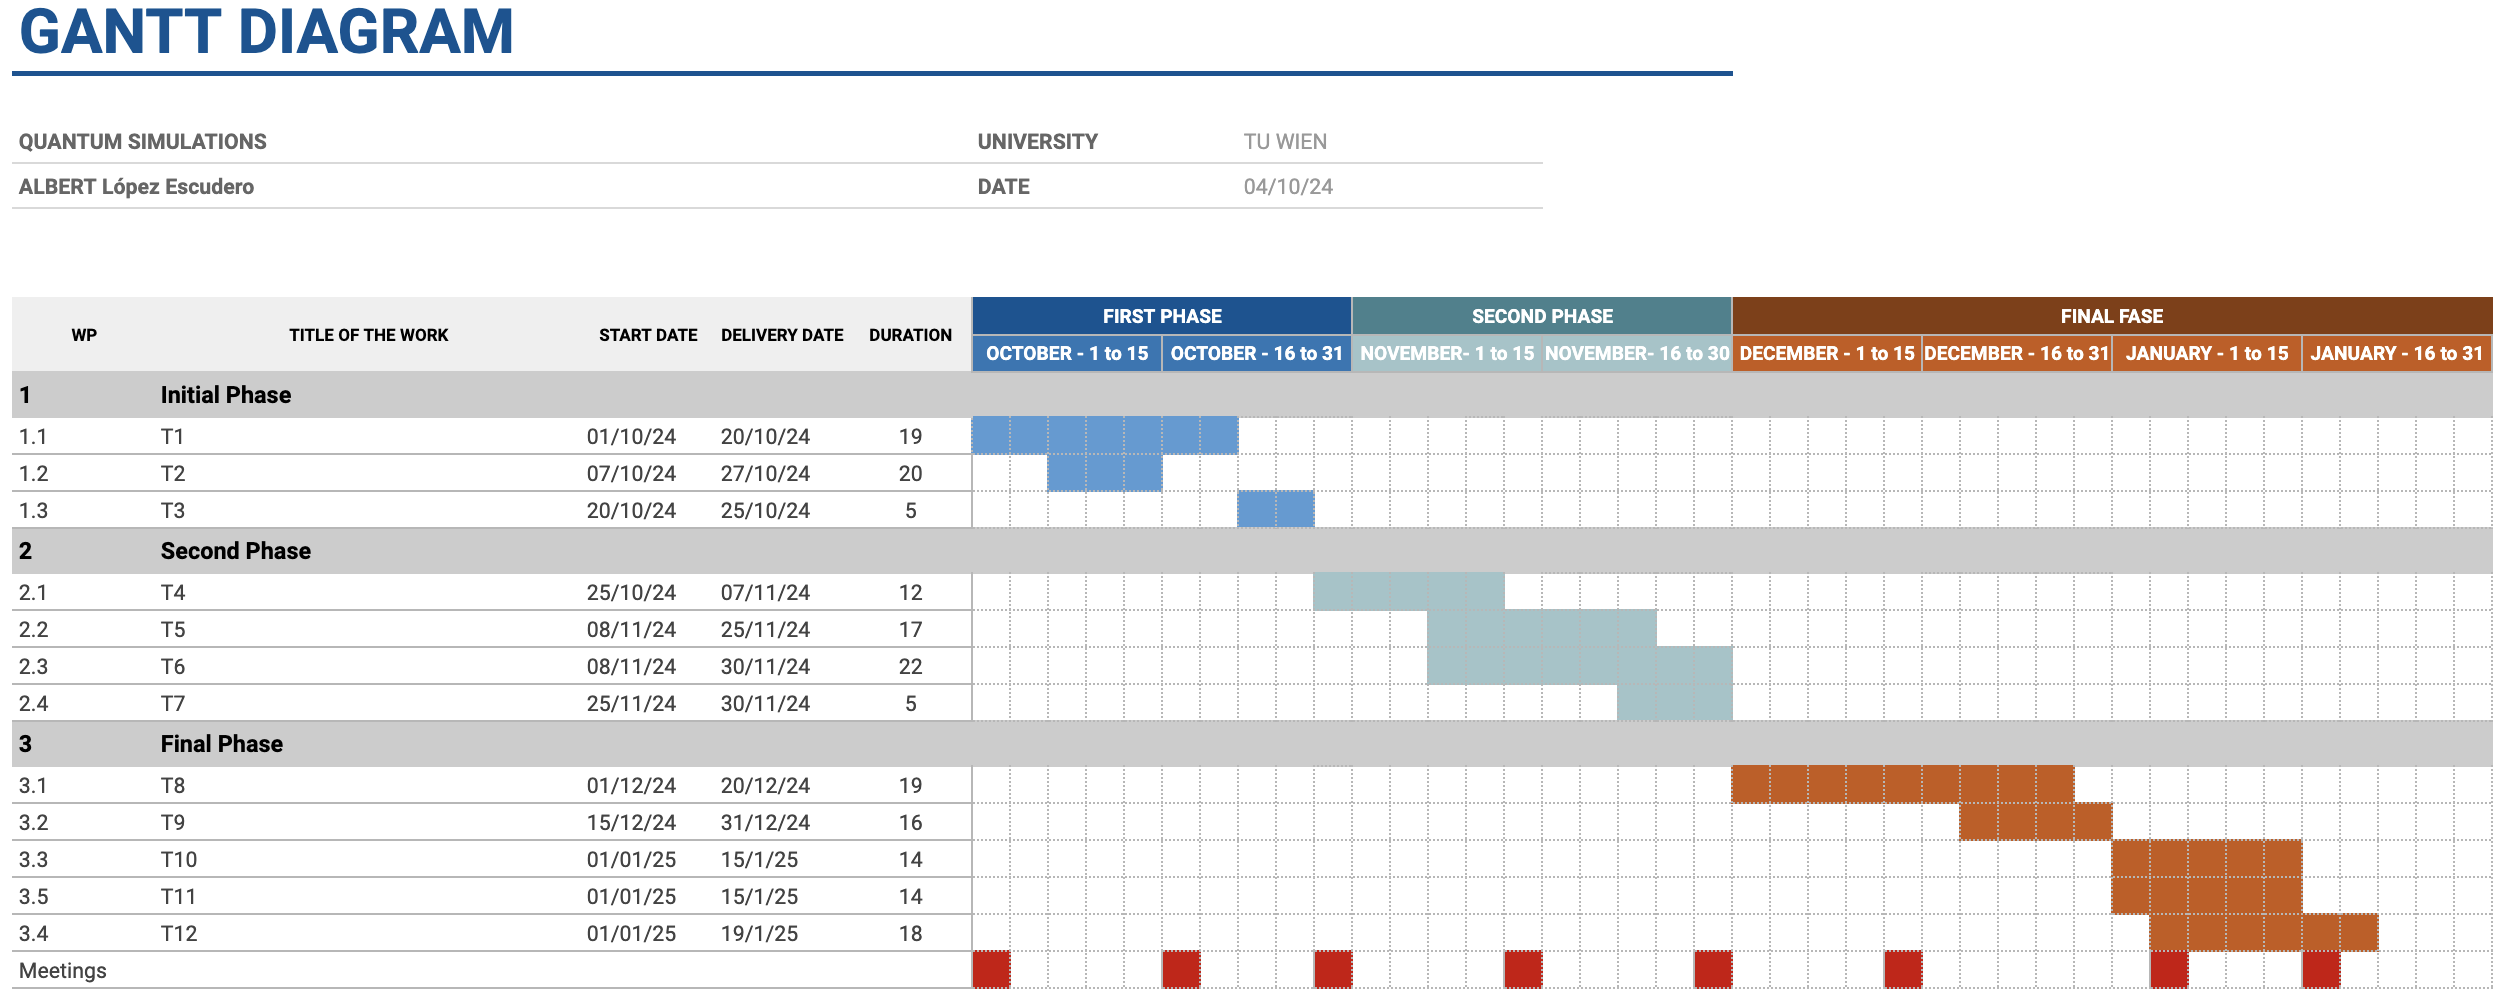
\includegraphics[width=1\textwidth]{img/Gantt_diagram.png}
  \caption{Project's Gantt diagram{\footnotesize{Gantt diagram of the project. For more information read the manual \cite{skalagantt} of Skala.}.}}
  \label{fig:gantt_diagram}
\end{figure}

